\documentclass[border=1pt]{standalone}
% ---------------------------------------------------------------------------
% Shared style for the MOSAIC / CRYSTAL TOMM figures.
% Compile each fig_*.tex with LuaLaTeX (standalone). Sized for acmart
% "acmsmall" (TOMM): \textwidth = 13.9 cm, so every figure is drawn at
% final size and is included with width=\textwidth (no rescaling of text).
% Fonts: Libertinus Sans + Inconsolata (acmart uses Libertine + Inconsolata).
% ---------------------------------------------------------------------------
\usepackage{fontspec}
\setmainfont{LibertinusSans}[Path=fonts/, Extension=.otf,
  UprightFont=*-Regular, BoldFont=*-Bold, ItalicFont=*-Italic]
\setmonofont{Inconsolata}[Path=fonts/, Extension=.otf,
  UprightFont=*-Regular, BoldFont=*-Bold, Scale=0.98]
\usepackage{unicode-math}
\setmathfont{LibertinusMath-Regular.otf}[Path=fonts/]

\usepackage{tikz}
\usetikzlibrary{positioning,fit,calc,arrows.meta,backgrounds,
  shapes.misc,shapes.geometric,decorations.pathreplacing,patterns.meta}

% Okabe-Ito palette (colour-blind safe) + tints -------------------------------
\definecolor{oiBlue}{HTML}{0072B2}
\definecolor{oiOrange}{HTML}{E69F00}
\definecolor{oiSky}{HTML}{56B4E9}
\definecolor{oiGreen}{HTML}{009E73}
\definecolor{oiVerm}{HTML}{D55E00}
\definecolor{oiPurple}{HTML}{CC79A7}
\definecolor{oiYellow}{HTML}{F0E442}
\definecolor{ink}{HTML}{1A1A1A}
\definecolor{muted}{HTML}{5C5C5C}
\definecolor{rule}{HTML}{9A9A9A}

\definecolor{oursFill}{HTML}{DDEBF7}
\definecolor{oursDraw}{HTML}{0072B2}
\definecolor{modFill}{HTML}{FCEFD2}
\definecolor{modDraw}{HTML}{B57600}
\definecolor{upFill}{HTML}{F1F1F1}
\definecolor{upDraw}{HTML}{7D7D7D}
\definecolor{failFill}{HTML}{FBE3D6}
\definecolor{okFill}{HTML}{D9F0E8}

% Sequence colours (as in the packetization study)
\definecolor{seqSOL}{HTML}{0072B2}
\definecolor{seqTHA}{HTML}{009E73}
\definecolor{seqLON}{HTML}{CC79A7}

% Typography -----------------------------------------------------------------
\newcommand{\figfont}{\fontsize{7.5}{9}\selectfont}
\newcommand{\smallfig}{\fontsize{6.5}{7.8}\selectfont}
\newcommand{\tinyfig}{\fontsize{6}{7.2}\selectfont}
\newcommand{\code}[1]{{\ttfamily #1}}

% Provenance encoding: colour AND line style (grayscale safe) ------------------
%  ours      = new component written by us      (blue, solid 0.9 pt)
%  modified  = upstream component we patched    (orange, dashed 0.8 pt)
%  upstream  = used unmodified / third party    (grey, solid 0.45 pt)
\tikzset{
  base/.style={rectangle, rounded corners=1.6pt, align=center,
    inner xsep=3pt, inner ysep=2.6pt, font=\figfont, text=ink,
    execute at begin node={\hyphenpenalty=10000\exhyphenpenalty=10000}},
  ours/.style={base, fill=oursFill, draw=oursDraw, line width=0.9pt},
  mod/.style={base, fill=modFill, draw=modDraw, line width=0.8pt,
    dash pattern=on 2.6pt off 1.4pt},
  up/.style={base, fill=upFill, draw=upDraw, line width=0.45pt},
  dead/.style={base, fill=white, draw=oiVerm, line width=0.6pt,
    dash pattern=on 1.2pt off 1.2pt, text=oiVerm},
  note/.style={font=\smallfig, text=muted, align=left,
    execute at begin node={\hyphenpenalty=10000\exhyphenpenalty=10000}},
  lab/.style={font=\smallfig\itshape, text=muted},
  zone/.style={draw=rule, line width=0.45pt, rounded corners=3pt,
    dash pattern=on 0.6pt off 1.1pt},
  zonetitle/.style={font=\figfont\bfseries, text=ink, anchor=west,
    inner xsep=2pt, inner ysep=1pt, fill=white, xshift=2.5mm},
  flow/.style={-{Stealth[length=4pt,width=3.2pt]}, line width=0.65pt,
    draw=ink},
  dflow/.style={flow, dash pattern=on 2pt off 1.4pt},
  ctrl/.style={-{Stealth[length=3.4pt,width=2.8pt]}, line width=0.5pt,
    draw=muted},
  failflow/.style={-{Stealth[length=4pt,width=3.2pt]}, line width=0.6pt,
    draw=oiVerm, dash pattern=on 1.4pt off 1.2pt},
  stepc/.style={circle, fill=ink, text=white, inner sep=0pt,
    minimum size=8.5pt, font=\tinyfig\bfseries},
  tag/.style={font=\tinyfig\bfseries, inner sep=1pt},
}

% Legend for the provenance encoding -------------------------------------------
\newcommand{\provlegend}[1]{% #1 = anchor coordinate (north west)
  \begin{scope}[shift={(#1)}]
    \node[ours, minimum width=6mm, minimum height=2.6mm, inner sep=0pt]
      (lg1) at (0,0) {};
    \node[anchor=west, font=\smallfig] at (lg1.east) {new (this work)};
    \node[mod, minimum width=6mm, minimum height=2.6mm, inner sep=0pt]
      (lg2) at (2.6,0) {};
    \node[anchor=west, font=\smallfig] at (lg2.east) {upstream, patched by us};
    \node[up, minimum width=6mm, minimum height=2.6mm, inner sep=0pt]
      (lg3) at (6.2,0) {};
    \node[anchor=west, font=\smallfig] at (lg3.east) {upstream / third party, unmodified};
  \end{scope}}

\newcommand{\bx}[2]{{\bfseries #1\par}\vspace{0.6pt}{\smallfig #2\par}}
\begin{document}
\figfont
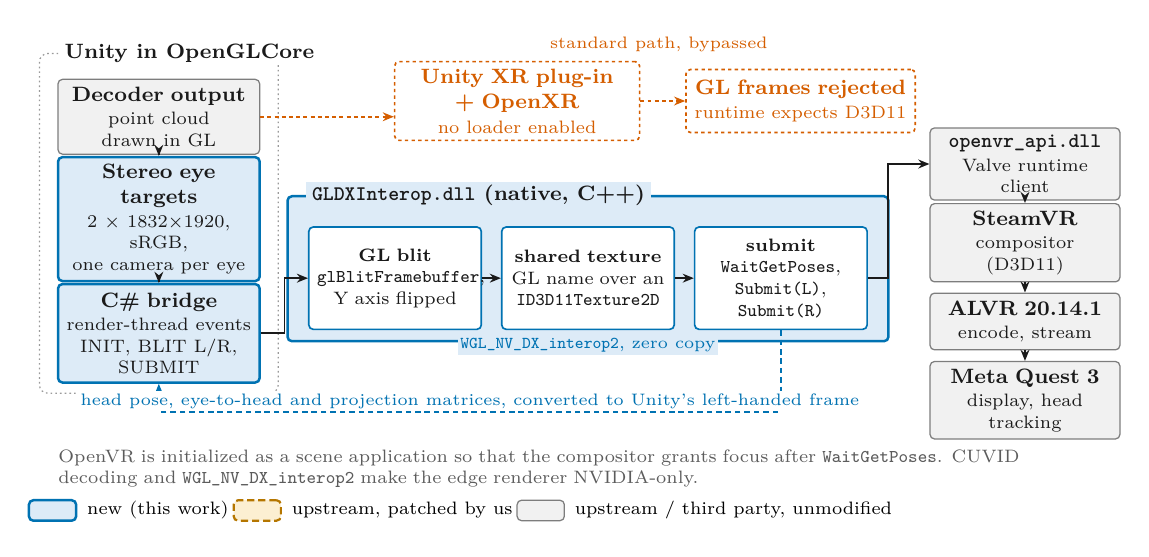
\begin{tikzpicture}[x=1cm,y=1cm]
  \tikzset{w/.style={text width=2.35cm, minimum height=0.95cm},
           pw/.style={base, fill=white, draw=oursDraw, line width=0.6pt,
              text width=1.98cm, minimum height=1.3cm, font=\smallfig},
           rw/.style={up, text width=2.2cm, minimum height=0.72cm}}

  % ---------------------------- Unity (OpenGLCore) ----------------------------
  \node[up, w] (dec) at (1.45,4.05) {\bx{Decoder output}{point cloud drawn in GL}};
  \node[ours, w] (rt) at (1.45,2.75) {\bx{Stereo eye targets}{2 × 1832×1920, sRGB,\\one camera per eye}};
  \node[ours, w, minimum height=1.25cm] (br) at (1.45,1.3) {\bx{C\# bridge}{render-thread events\\INIT, BLIT L/R,\\SUBMIT}};
  \draw[flow] (dec) -- (rt);
  \draw[flow] (rt) -- (br);
  \begin{scope}[on background layer]
    \node[zone, fit=(dec)(rt)(br), inner sep=2.2mm, yshift=1mm] (zu) {};
  \end{scope}
  \node[zonetitle] at (zu.north west) {Unity in OpenGLCore};

  % ---------------------------- GLDXInterop.dll --------------------------------
  \node[pw] (bl) at (4.45,2.0) {\textbf{GL blit}\\\code{glBlitFramebuffer},\\Y axis flipped};
  \node[pw] (ix) at (6.9,2.0) {\textbf{shared texture}\\GL name over an\\\code{ID3D11Texture2D}};
  \node[pw] (sb) at (9.35,2.0) {\textbf{submit}\\\code{WaitGetPoses},\\\code{Submit(L)}, \code{Submit(R)}};
  \draw[flow] (bl) -- (ix);
  \draw[flow] (ix) -- (sb);
  \node[font=\tinyfig, text=oiBlue, anchor=north, fill=oursFill, inner sep=1pt] at ($(ix.south)+(0,-0.06)$) {\code{WGL\_NV\_DX\_interop2}, zero copy};
  \begin{scope}[on background layer]
    \node[ours, fit=(bl)(ix)(sb), inner sep=2.6mm, yshift=1.2mm, fill=oursFill] (zp) {};
  \end{scope}
  \node[zonetitle, fill=oursFill] at (zp.north west) {\code{GLDXInterop.dll} (native, C++)};
  \draw[flow] (br.east) -- ++(0.3,0) |- (bl.west);

  % ---------------------------- OpenVR delivery --------------------------------
  \node[rw] (ovr) at (12.45,3.45) {\bx{\code{openvr\_api.dll}}{Valve runtime client}};
  \node[rw] (svr) at (12.45,2.45) {\bx{SteamVR}{compositor (D3D11)}};
  \node[rw] (alvr) at (12.45,1.45) {\bx{ALVR 20.14.1}{encode, stream}};
  \node[rw] (q3) at (12.45,0.45) {\bx{Meta Quest 3}{display, head tracking}};
  \draw[flow] (sb.east) -- ++(0.25,0) |- (ovr.west);
  \draw[flow] (ovr) -- (svr); \draw[flow] (svr) -- (alvr); \draw[flow] (alvr) -- (q3);

  % ---------------------------- bypassed OpenXR path ---------------------------
  \node[dead, text width=2.9cm, minimum height=0.8cm] (xr) at (6.0,4.25)
    {{\bfseries Unity XR plug-in + OpenXR}\par{\smallfig no loader enabled}};
  \node[dead, text width=2.7cm, minimum height=0.8cm] (drop) at (9.6,4.25)
    {{\bfseries GL frames rejected}\par{\smallfig runtime expects D3D11}};
  \draw[failflow] (dec.east) -- (xr.west |- dec.east);
  \draw[failflow] (xr) -- (drop);
  \node[font=\tinyfig, text=oiVerm, anchor=south] at ($(xr.north)!0.5!(drop.north)+(0,0.04)$) {standard path, bypassed};

  % ---------------------------- pose feedback ----------------------------------
  \draw[dflow, draw=oiBlue] (sb.south) -- (sb.south |- 0,0.3) -- (1.45,0.3) -- (br.south);
  \node[font=\tinyfig, text=oiBlue, anchor=south, fill=white, inner sep=1pt] at (5.4,0.3)
    {head pose, eye-to-head and projection matrices, converted to Unity's left-handed frame};

  % ---------------------------- notes -----------------------------------------
  \node[note, anchor=north west, text width=13.2cm] at (0.05,-0.05)
    {OpenVR is initialized as a scene application so that the compositor grants focus after \code{WaitGetPoses}. CUVID decoding and \code{WGL\_NV\_DX\_interop2} make the edge renderer NVIDIA-only.};

  \provlegend{0.1,-0.95}
\end{tikzpicture}
\end{document}
